\documentclass[10pt]{article}
\usepackage[ngerman]{babel}
\usepackage[utf8]{inputenc}
\usepackage[T1]{fontenc}
\usepackage{amsmath}
\usepackage{amsfonts}
\usepackage{amssymb}
\usepackage[version=4]{mhchem}
\usepackage{stmaryrd}
\usepackage{graphicx}
\usepackage[export]{adjustbox}
\graphicspath{ {./images/} }

\begin{document}
\section*{CT1 Übungsaufgaben}
\section*{Unterprogramme und Stack}
\section*{Aufgabe}
Im folgenden Assembler-Programm werden die vier Unterprogramme procA, procB, procC und procD aufgerufen und einige Register mit PUSH gesichert und zurückgeladen. Zu Beginn des Programmes steht der Stackpointer (SP) auf 0x20000660.\\
Bestimmen Sie zu den angegebenen Zeitpunkten Z1. . . Z4 den Inhalt des Stacks. Schreiben Sie daneben die Bedeutung des Stack-Inhaltes, z.B. Inhalt R1 von procX oder ret adr von procY).

\begin{center}
\begin{tabular}{|c|c|c|c|}
\hline
28 & endless &  &  \\
\hline
29 0x0800079C 490D & LDR & $\mathrm{R} 1,=0 \times 10203040$ &  \\
\hline
$300 \times 0800079 \mathrm{4}$ 40E & LDR & $\mathrm{R} 2,=0 \times 50607080$ &  \\
\hline
31 0x080007A0 F000 F804 & BL & procA &  \\
\hline
32 0x080007A4 F000 F807 & BL & procB &  \\
\hline
33 0x080007A8 E7F8 & B & endless &  \\
\hline
$340 \times 080007 A A 0000$ & ALIGN &  &  \\
\hline
39 & procA &  &  \\
\hline
40 0x080007AC B406 & PUSH & \{R1, R2\} &  \\
\hline
41 &  &  & ; <------------- (Z1) \\
\hline
42 0x080007AE 490B & LDR & R1, =0xAABBCCDD &  \\
\hline
43 0x080007B0 4A0B & LDR & R2, =0xEEFF1020 &  \\
\hline
44 0x080007B2 BC06 & POP & \{R1, R2\} &  \\
\hline
45 0x080007B4 4770 & BX & LR &  \\
\hline
46 &  &  &  \\
\hline
47 & procB &  &  \\
\hline
48 0x080007B6 B506 & PUSH & \{R1, R2, LR \} &  \\
\hline
49 &  &  & ; <------------- (Z2) \\
\hline
50 0x080007B8 490A & LDR & R1, $=0 \times 11223344$ &  \\
\hline
51 0x080007BA 4A0B & LDR & R2, $=0 \times 55667788$ &  \\
\hline
52 0x080007BC F000 F801 & BL & procC &  \\
\hline
53 0x080007C0 BD06 & POP & \{R1, R2, PC\} &  \\
\hline
54 &  &  &  \\
\hline
55 & procC &  &  \\
\hline
56 0x080007C2 B506 & PUSH & \{R1, R2, LR \} &  \\
\hline
57 &  &  & ; <------------- (Z3) \\
\hline
$580 \times 080007 \mathrm{C} 44909$ & LDR & R1, $=0 \times 11111111$ &  \\
\hline
59 0x080007C4 4A0A & LDR & $\mathrm{R} 2,=0 \times 2222222$ &  \\
\hline
60 0x080007C8 F000F801 & BL & procD &  \\
\hline
61 0x080007CC BD06 & POP & \{R1, R2, PC \} &  \\
\hline
62 &  &  & ; <------------- (Z4) \\
\hline
\end{tabular}
\end{center}

\begin{center}
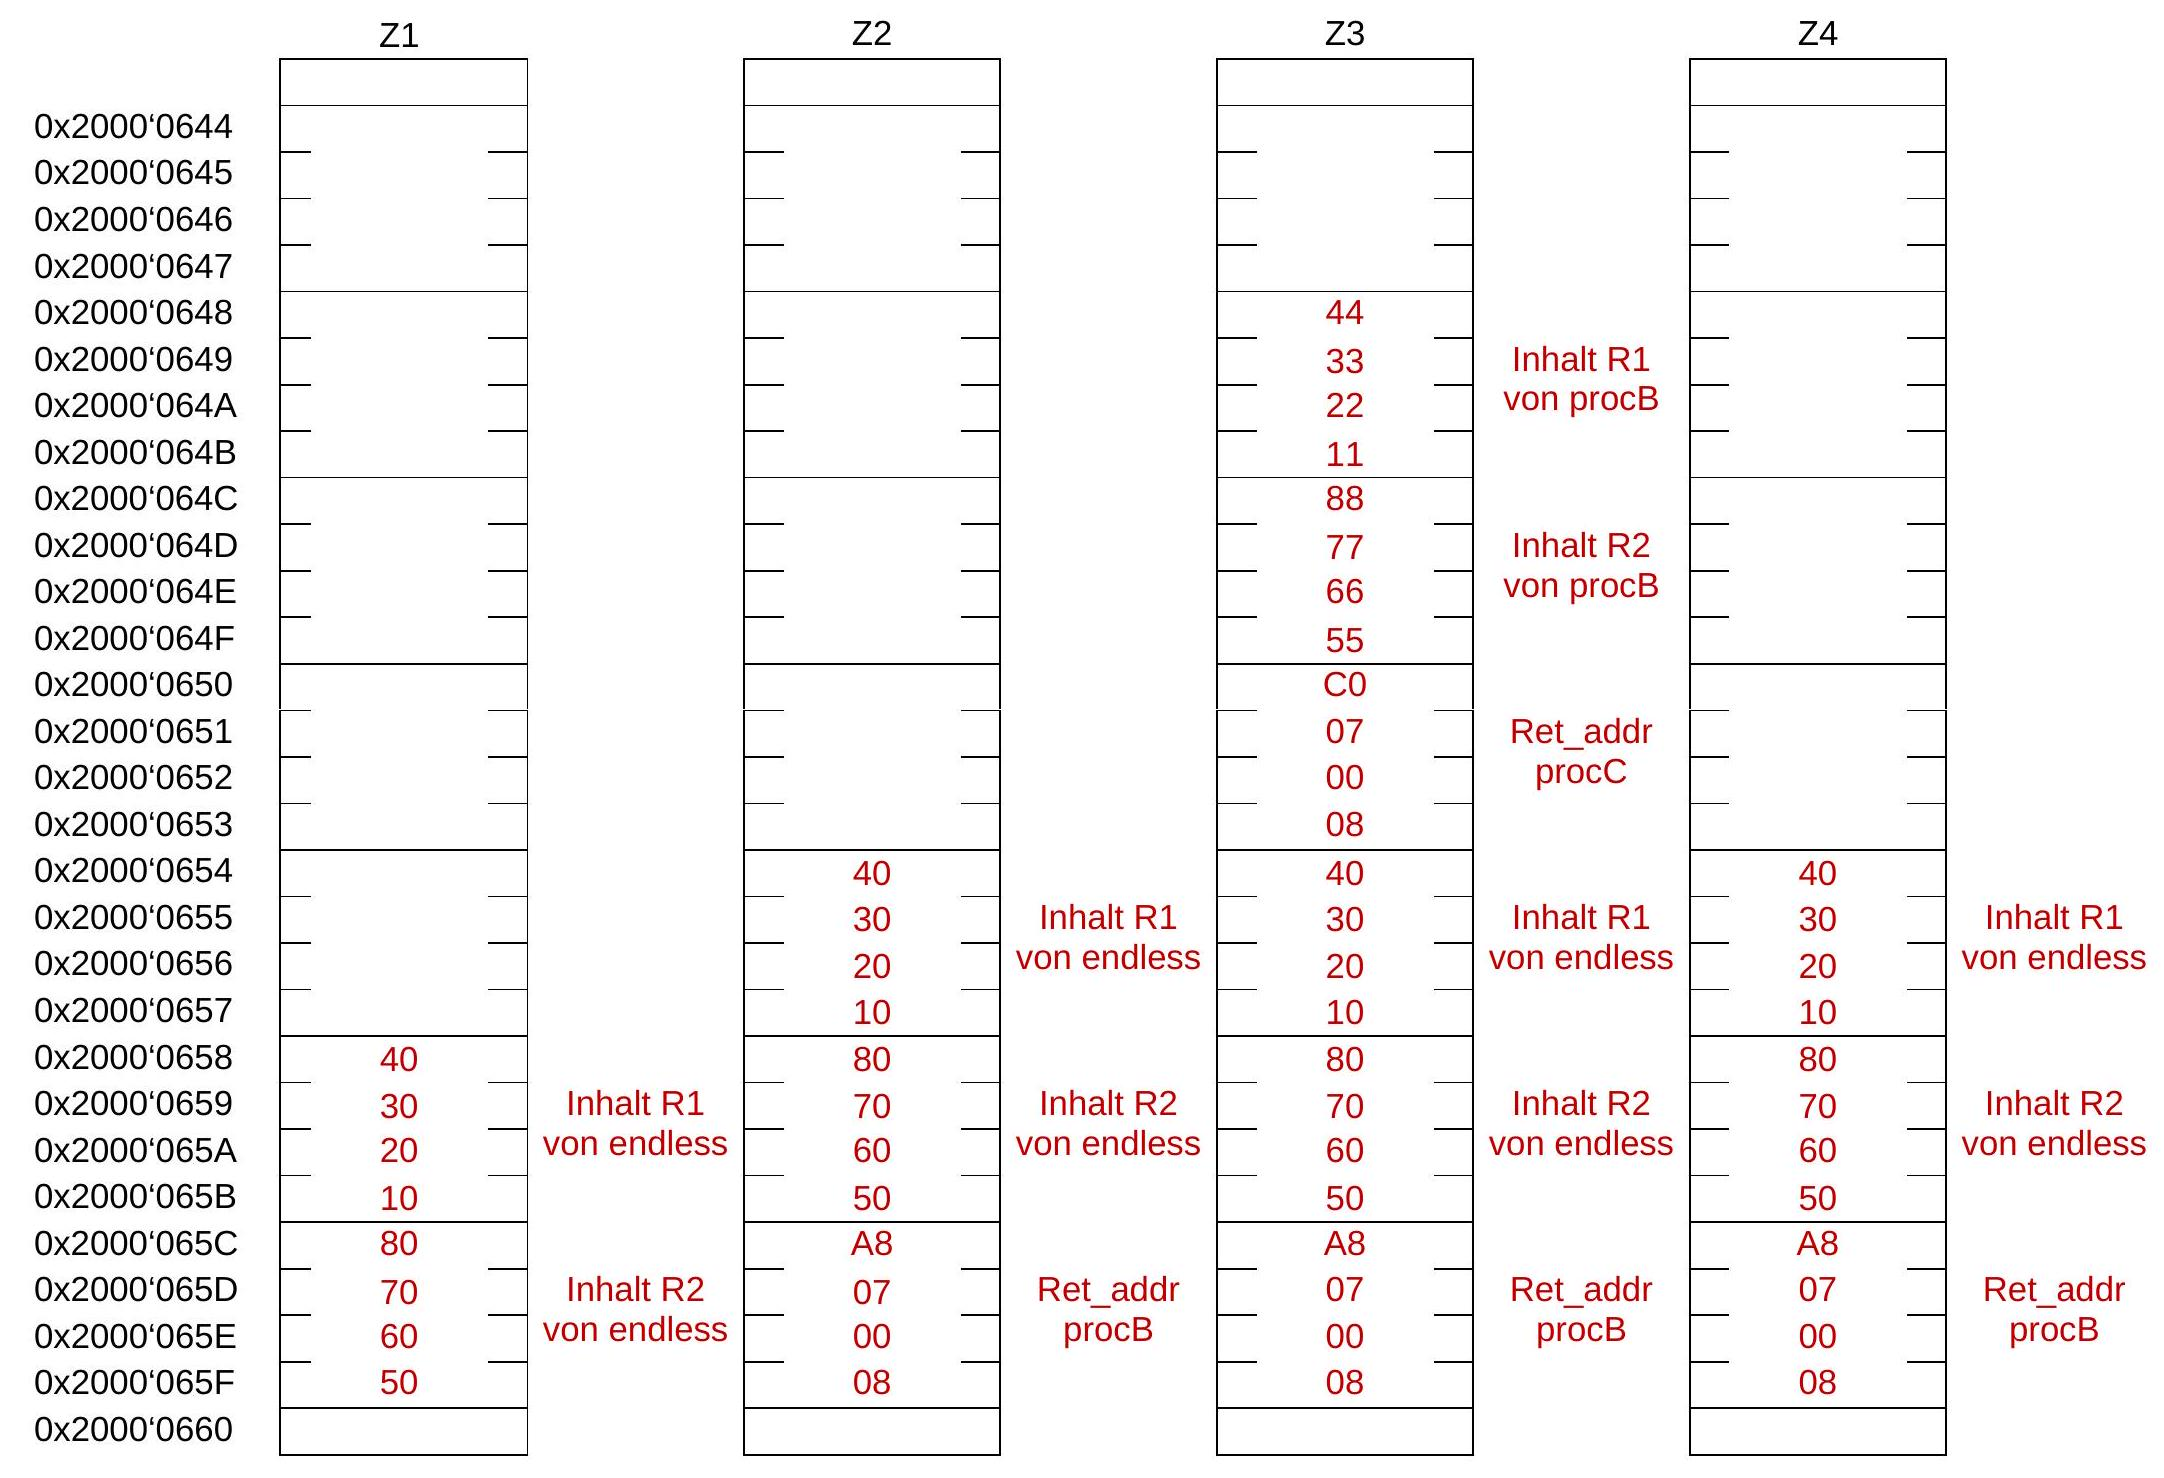
\includegraphics[width=\linewidth]{images/2025_01_02_88a231b00f1bec111bb0g-2}
\end{center}


\end{document}